% Part: sets-functions-relations
% Chapter: relations
% Section: graphs

\documentclass[../../../include/open-logic-section]{subfiles}

\begin{document}

\olfileid{sfr}{rel}{grp}
\olsection{గ్రాఫులు}

ఒక \emph{గ్రాఫు} అనేది బిందువులను అంచులతో కలిపి చూపే చిత్రం.
ఆ బిందువులను “నోడ్‌లు” లేదా “శీర్షాలు” అంటారు.
వివిక్త గణితంలోనూ కంప్యూటర్ శాస్త్రంలోనూ గ్రాఫులు విస్తృతంగా
ఉపయోగపడతాయి. వివిధ రకాల వలయాల వంటి మూర్త విషయాల నుంచి,
నిర్ణయాల వల్ల కలగగల ఫలితాల వంటి అమూర్త నిర్మాణాల వరకు,
సంబంధాలనూ నిర్మాణాలనూ సూచించడానికి, దృశ్యరూపంలో చూపడానికి అవి
ఎంతో ఉపయోగకరం. సాహిత్యంలో వేర్వేరు రకాల గ్రాఫులు ఉన్నాయి.
ఉదాహరణకు అంచులకు దిశలు ఉన్నాయా లేదా, గుర్తింపులు ఉన్నాయా లేదా,
ఒక శీర్షం నుంచి అదే శీర్షానికి అంచు ఉండవచ్చా లేదా, ఒకే శీర్షాల
మధ్య అనేక అంచులు ఉండవచ్చా లేదా అన్న విషయాలలో అవి భిన్నంగా ఉంటాయి.
\emph{దిశా గ్రాఫులకు} సంబంధాలతో ప్రత్యేకమైన అనుబంధం ఉంది.

\begin{defn}[దిశా గ్రాఫు]
ఒక \emph{దిశా గ్రాఫు} $G = \tuple{V, E}$లో
\emph{శీర్షాల} సమితి $V$, \emph{అంచుల} సమితి $E \subseteq V^2$ ఉంటాయి.
\end{defn}

\begin{explain}
మన నిర్వచనం ప్రకారం, గ్రాఫు అంటే ఒక సమితి, దానిపైన ఒక సంబంధం.
గ్రాఫుల గురించి మాట్లాడేటప్పుడు వాటిని చిత్రాలుగా చూపుతారని
ఆశించడం సహజమే: $\tuple{v_1, v_2} \in E$ అయితే, అయితేనే
$v_1$, $v_2$ అనే రెండు శీర్షాలను బాణంతో కలిపి గ్రాఫును గీయవచ్చు.
ఒక సంబంధానికీ గ్రాఫుకూ ఉన్న ఏకైక తేడా ఏమిటంటే, గ్రాఫు శీర్షాల
సమితిని నిర్దేశిస్తుంది; అంటే గ్రాఫులో ఇతర శీర్షాలతో కలవని
ఒంటరి శీర్షాలు ఉండవచ్చు. ముఖ్యమైన విషయం మాత్రం ఇది:
$X$ అనే సమితిపై ప్రతి సంబంధం $R$నూ $\tuple{X, R}$ అనే
దిశా గ్రాఫుగా చూడవచ్చు. తిరుగుగా, $\tuple{V, E}$ అనే దిశా గ్రాఫును,
$V$ సమితిని స్పష్టంగా నిర్దేశించిన $E \subseteq V^2$ సంబంధంగా చూడవచ్చు.
\end{explain}

\begin{ex}
$V = \{1, 2, 3, 4\}$,
$E = \{\tuple{1,1}, \allowbreak \tuple{1, 2}, \allowbreak \tuple{1, 3},
\allowbreak \tuple{2, 3}\}$ ఉన్న $\tuple{V, E}$ గ్రాఫు ఇలా కనిపిస్తుంది:
\begin{align*}
& 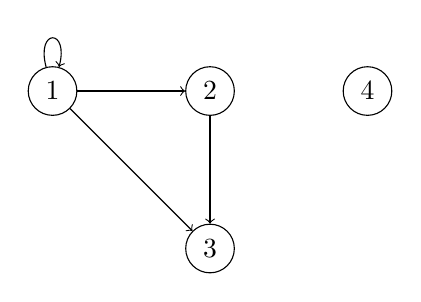
\begin{tikzpicture}[->,node distance=2cm]
  \node[draw,circle] (A) {$1$};
  \node[draw,circle] (B) [right of=A] {$2$};
  \node[draw,circle] (C) [below of=B] {$3$};
  \node[draw,circle] (D) [right of=B] {$4$};
  \draw (A) to [loop above]  (A);
  \draw (A) to  (B);
  \draw (A) to  (C);
  \draw (B) to  (C);
  \end{tikzpicture}
\intertext{ఇది $V' = \{1, 2, 3\}$ ఉన్న $\tuple{V', E}$
  గ్రాఫుకు భిన్నమైనది. ఆ గ్రాఫు ఇలా కనిపిస్తుంది:}
& 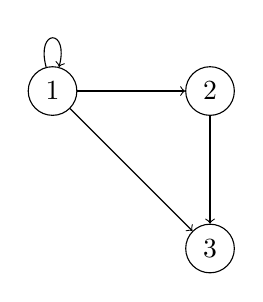
\begin{tikzpicture}[->,node distance=2cm]
  \node[draw,circle] (A) {$1$};
  \node[draw,circle] (B) [right of=A] {$2$};
  \node[draw,circle] (C) [below of=B] {$3$};
  \draw (A) to [loop above]  (A);
  \draw (A) to  (B);
  \draw (A) to  (C);
  \draw (B) to  (C);
  \end{tikzpicture}
\end{align*}
\end{ex}

\begin{prob}
  $\{1, 2, 3, 4\}$ అనే సమితిపై చిన్నది-లేదా-సమానమైనది అనే
  $\le$ సంబంధాన్ని గ్రాఫుగా పరిగణించి, దాని చిత్రాన్ని గీయండి.
\end{prob}

\end{document}
